%! Author = melek
%! Date = 9.06.2022

% Preamble
\documentclass[11pt]{article}

% Packages
\usepackage{amsmath}
\DeclareMathOperator*{\argmax}{argmax}

\usepackage{graphicx}
\usepackage{amssymb}
\graphicspath{ {../images/} }

% Document
\begin{document}

    \maketitle
    \setcounter{section}{6}


    \section{Exercises}

    \subsection{Question}

    In Chapter 6 we noted that the Monte Carlo error can be written as the sum of TD errors (6.6) if the value estimates don’t change from step to step.
    Show that the n-step error used in (7.2) can also be written as a sum TD errors (again if the value estimates don’t change) generalizing the earlier result.

    \subsection*{Answer}

    Value estimates are assumed not to change thus we can omit value estimate subscripts such that $ V_t(S_t) = V_{t+1}(S_t)$.

    n-step TD Error used in 7.2  is:
    \newline
    $G_{t:t+n} - V(S_t) = R_{t+1} + \gamma G_{t+1:t+n} - V(S_t) $
    \newline
    $G_{t:t+n} - V(S_t) = R_{t+1} + \gamma V(S_{t+1}) - V(S_t) + \gamma G_{t+1:t+n} - \gamma V(S_{t+1}) $
    \newline
    $G_{t:t+n} - V(S_t) = \delta_t + \gamma ( G_{t+1:t+n} - V(S_{t+1}) ) $
    \newline
    $G_{t:t+n} - V(S_t) = \delta_t + \gamma \delta_{t+1} + \gamma^2 ( G_{t+2:t+n} - V(S_{t+2}) ) $
    \newline
    $G_{t:t+n} - V(S_t) = \sum_{k=t}^{t+n-1} \gamma^{k-t} \delta_k  $

    \subsection{Question}
    (programming) With an n-step method, the value estimates do change from step to step, so an algorithm that used the sum of TD errors (see previous exercise) in place of the error in (7.2) would actually be a slightly different algorithm.
    Would it be a better algorithm or a worse one?
    Devise and program a small experiment to answer this question empirically.

    \subsection*{Answer}

    The chart above shows regular n-step TD with different n parameters.
    The chart below shows the same configuration with unchanged value functions.
    Value function updates are applied only after an episode terminates.

    Using sum of TD errors as in place of the error in 7.2 performs worse in all n and $\alpha$ values.

    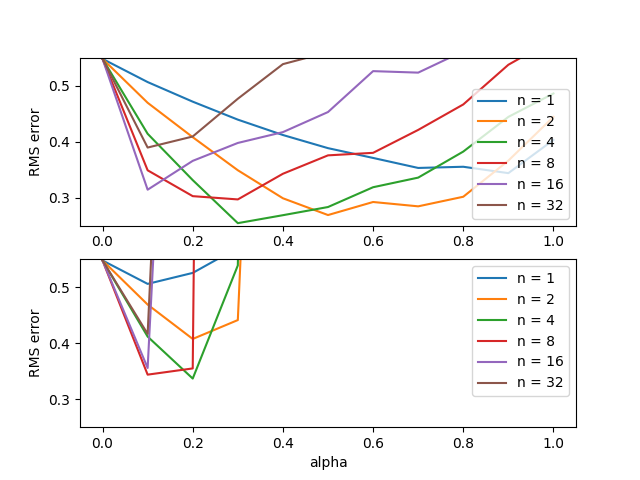
\includegraphics[scale=1]{figure_7_2}

\end{document}


